\documentclass[a4paper,12pt]{article}

\usepackage{times}
\usepackage{changepage}
\usepackage{setspace}
\usepackage{sidecap}
\usepackage{graphicx}
\usepackage[document]{ragged2e}
\usepackage{amsmath}

\begin{document}
\pagenumbering{gobble}
\setlength{\parindent}{0em}
\doublespacing

\begin{center}
{\huge PACCMAN Tutorial}
\end{center}

\bigskip
\bigskip


This document is a tutorial to explain how to use the PACCMAN program. It is expected that users will have a package manager such as Anaconda or another program with Numpy, Scipy, Matplotlib, etc. installed.

\medskip

PACCMAN is set by default to import data from the "basedata.py" file. A selection of this file is seen in the picture below. This file can be changed, or line 10 in the "paccman.py" file can be changed to import different inputs.

\begin{center}
\begin{figure}[h]
\centering
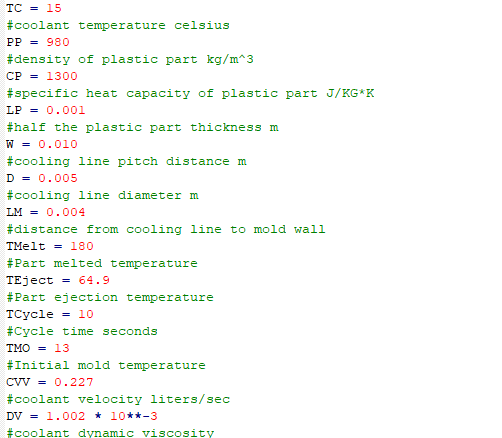
\includegraphics{tutorialimage1.png}
\end{figure}
\end{center}

\clearpage

After the input data is set, the program is ready to run. Using Anaconda (or something similar), navigate to the directory the program is saved in and run the following command:

\begin{center}
\begin{figure}[h]
\centering
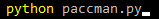
\includegraphics{tutorialimage2.png}
\end{figure}
\end{center}

The program will then ask the following question:

\begin{center}
\begin{figure}[h]
\centering
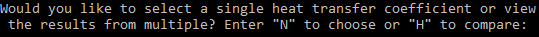
\includegraphics{tutorialimage3.png}
\end{figure}
\end{center}

Choosing "N" will cause the program to prompt the user to select a heat transfer coefficient correlation. The options are "D" for Ditus-Boelter, "G" for Gnielinski, and "S" for Sieder-Tate. Selecting "H" will compare all three.

\medskip

Once the heat transfer coefficient correlation is set, the user has the option to save a picture of the average temperature over time graph:

\begin{center}
\begin{figure}[h]
\centering
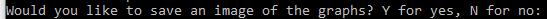
\includegraphics{tutorialimage4.png}
\end{figure}
\end{center}

\clearpage

The following image is an example of option "H", to compare the heat transfer coefficient correlations:

\begin{center}
\begin{figure}[h]
\centering
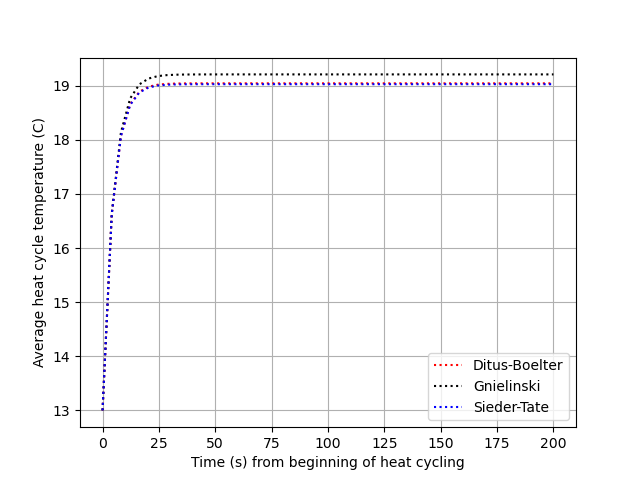
\includegraphics{tutorialimage5.png}
\end{figure}
\end{center}

\clearpage

The following image is an example of option "N", to only show the selected heat transfer coefficient correlation:

\begin{center}
\begin{figure}[h]
\centering
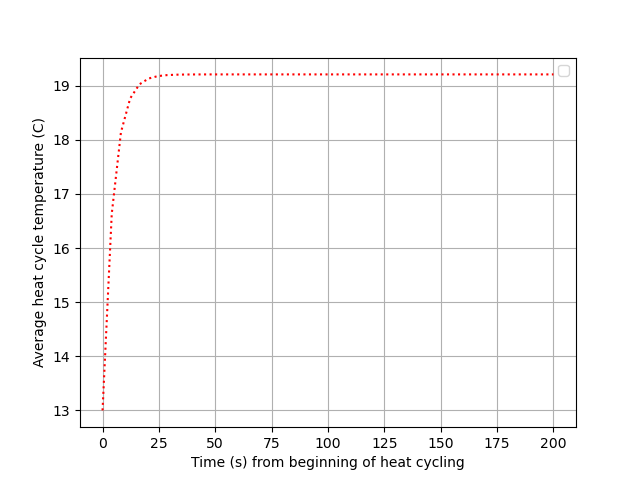
\includegraphics{tutorialimage6.png}
\end{figure}
\end{center}

\end{document}